	\section{Proposal}
    We propose to build a tool which will visualize the spatiotemporal values of the dataset, visuliaze the output of Machine Learning model and also visualize the points where the mismatches of testing and machine data occur based on the results of the Machine Learning model. We will be using Multi Label Classification Machine Learning Algorithms like support vector machines and existing neural networks to classify the audio files into various categorical sounds. Based on the results of ML model, we will dwell into understanding the mismatches which occur between the annotated and machine predicted data and analyze the causes behind it. 
    
    The technologies which we plan to use in order to build this tool would be ReactJS on the front-end and Django on the back-end. We are using ReactJS because of its component based architecture and its rich support with D3.js, Open Layers. Similarly, Django allows us to run various python libraries to process the data and creation of REST API's(representational state transfer application programming interface) to communicate with the front-end. 
   
   	We have divided the process of building this tool into four stages(see Figure 2) namely data preprocessing state where we process the audio files, Modeling stage where we apply the classification models on the dataset and create REST API's to interact with the front-end, Visualization stage where we visualize the results of machine learning model on the front-end, component building stage where we build components which allows the user to pick spatial and temporal values of various sound samples and display the results on a map.
   	
    This tool would be useful to authorities who monitor sounds around the city which will allow them to pinpoint the location of sound origin.
	\begin{figure}[h!]
	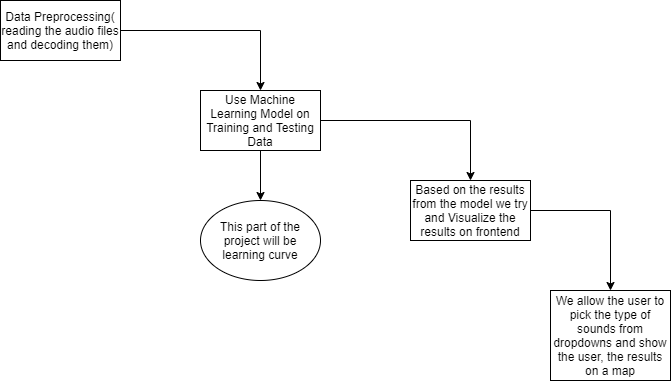
\includegraphics[width=9cm]{figure2}
	\caption{ Work flow diagram}
	\end{figure}
	
	
